\section{Figures}
\subsection{1f)}\label{app:fig}

\begin{figure}
\hspace{-2.8cm}
\begin{tabular}{cc}
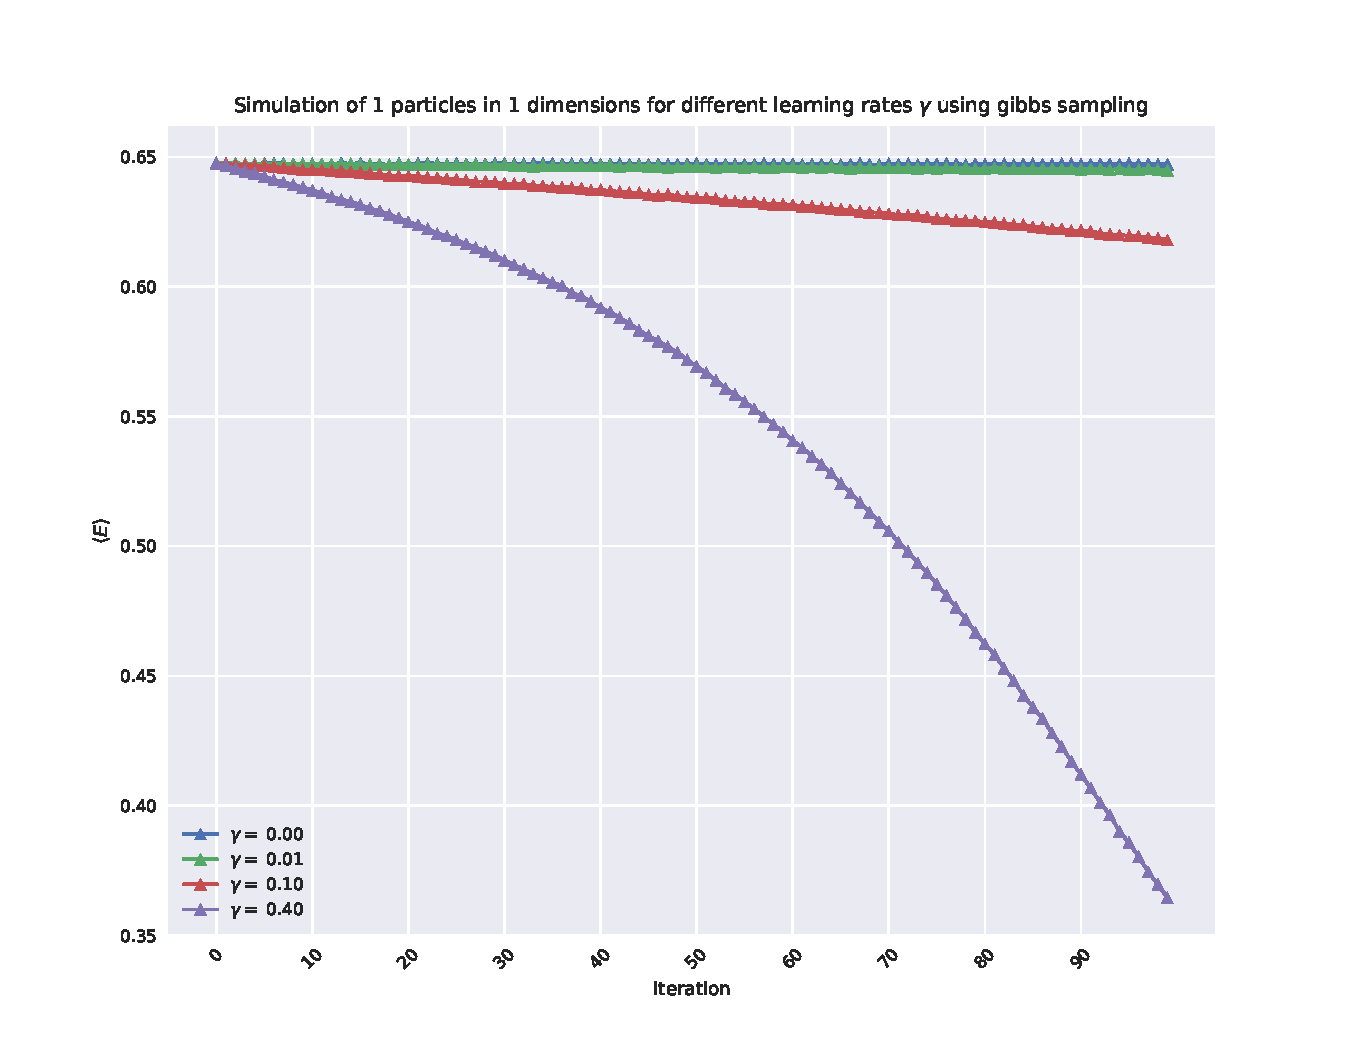
\includegraphics[width = 0.5\paperwidth]{figures/gibbs_1p_1d_N2.pdf} & 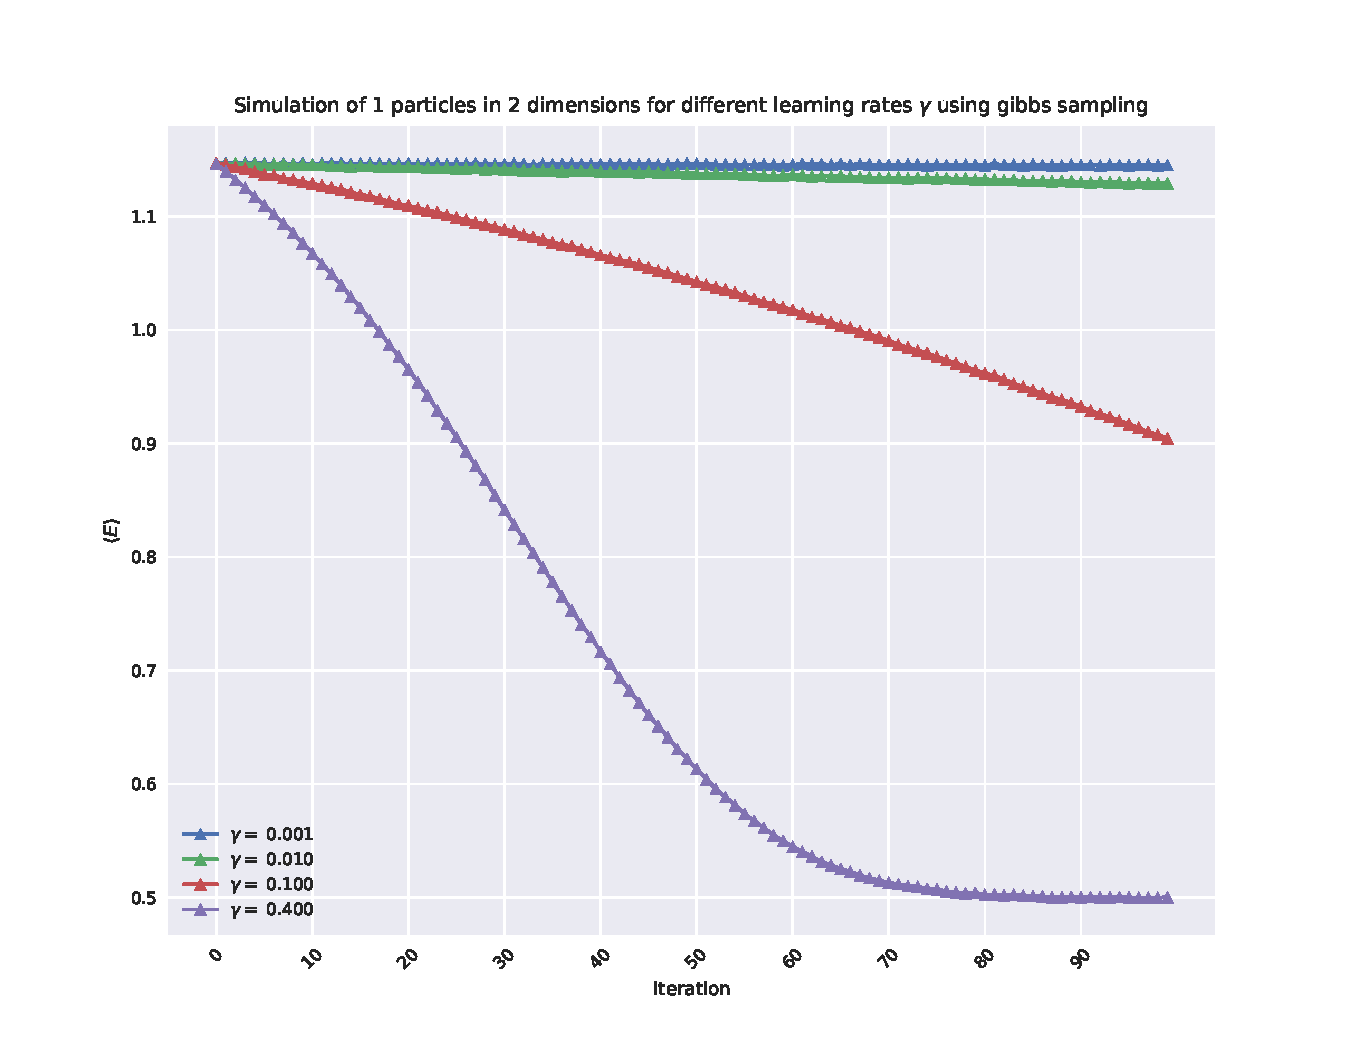
\includegraphics[width = 0.5\paperwidth]{figures/gibbs_1p_2d_N3.pdf} \\
\multicolumn{2}{c}{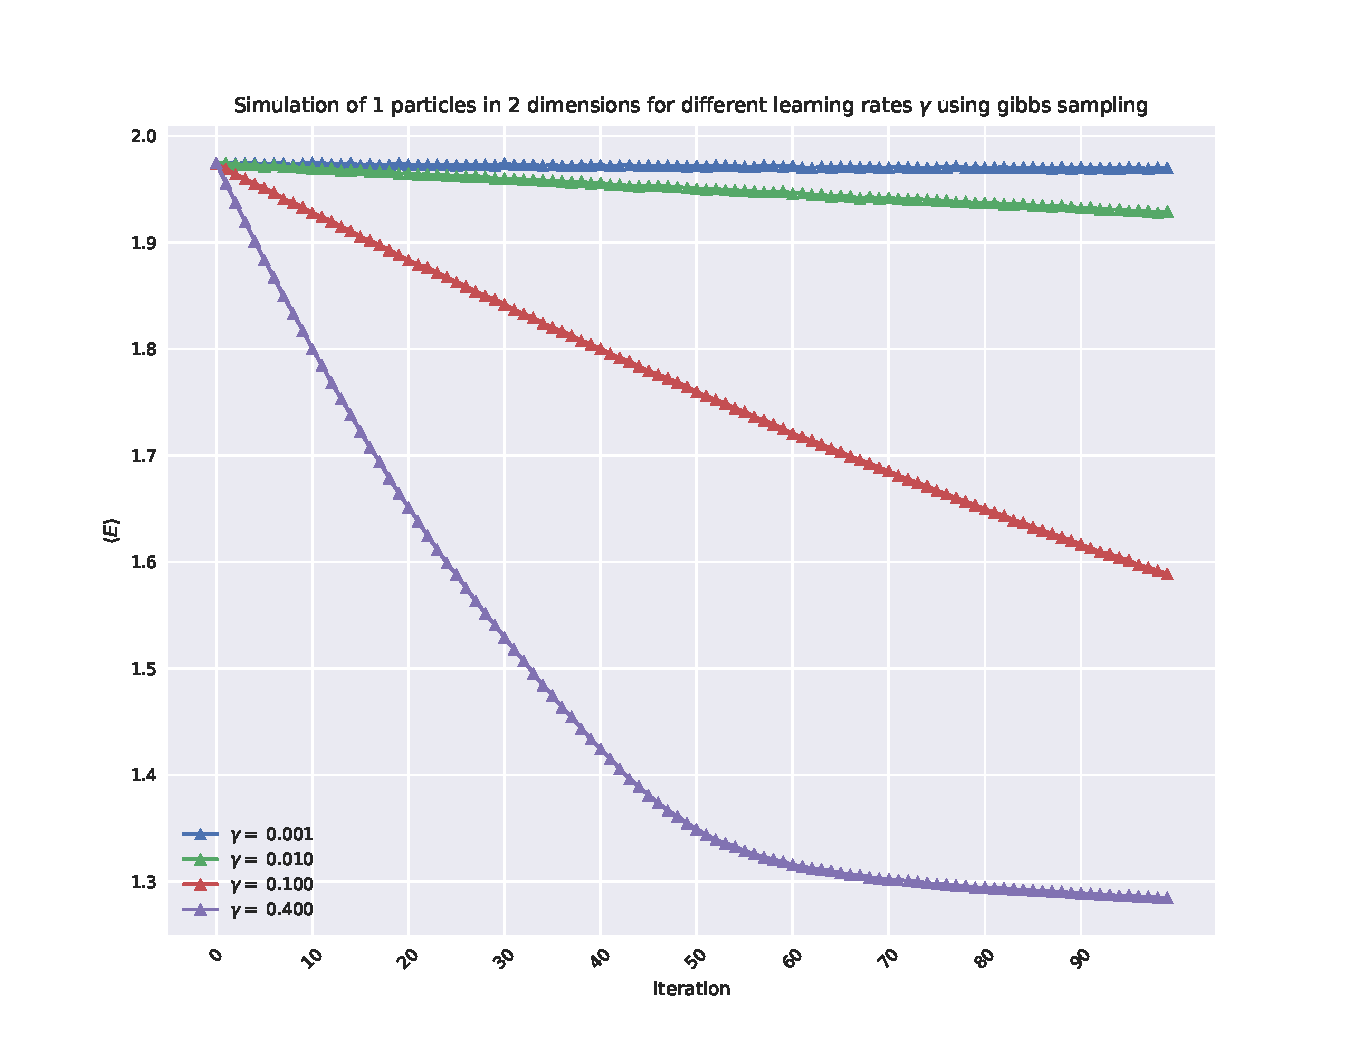
\includegraphics[width=0.5\paperwidth]{figures/gibbs_1p_3d_N4.pdf} }
\end{tabular}
\caption{Plots for simulations with 1 particle and 1-3 dimensions using Gibbs sampling with different training rate values. Number of simulations for optimizing parameters are showed in x-axis.(The lowest figure is for 1 particle in 3 dimensions, wrong title.)}
\label{fig:1f_1}
\end{figure}

\begin{figure}
\hspace{-2.8cm}
\begin{tabular}{cc}
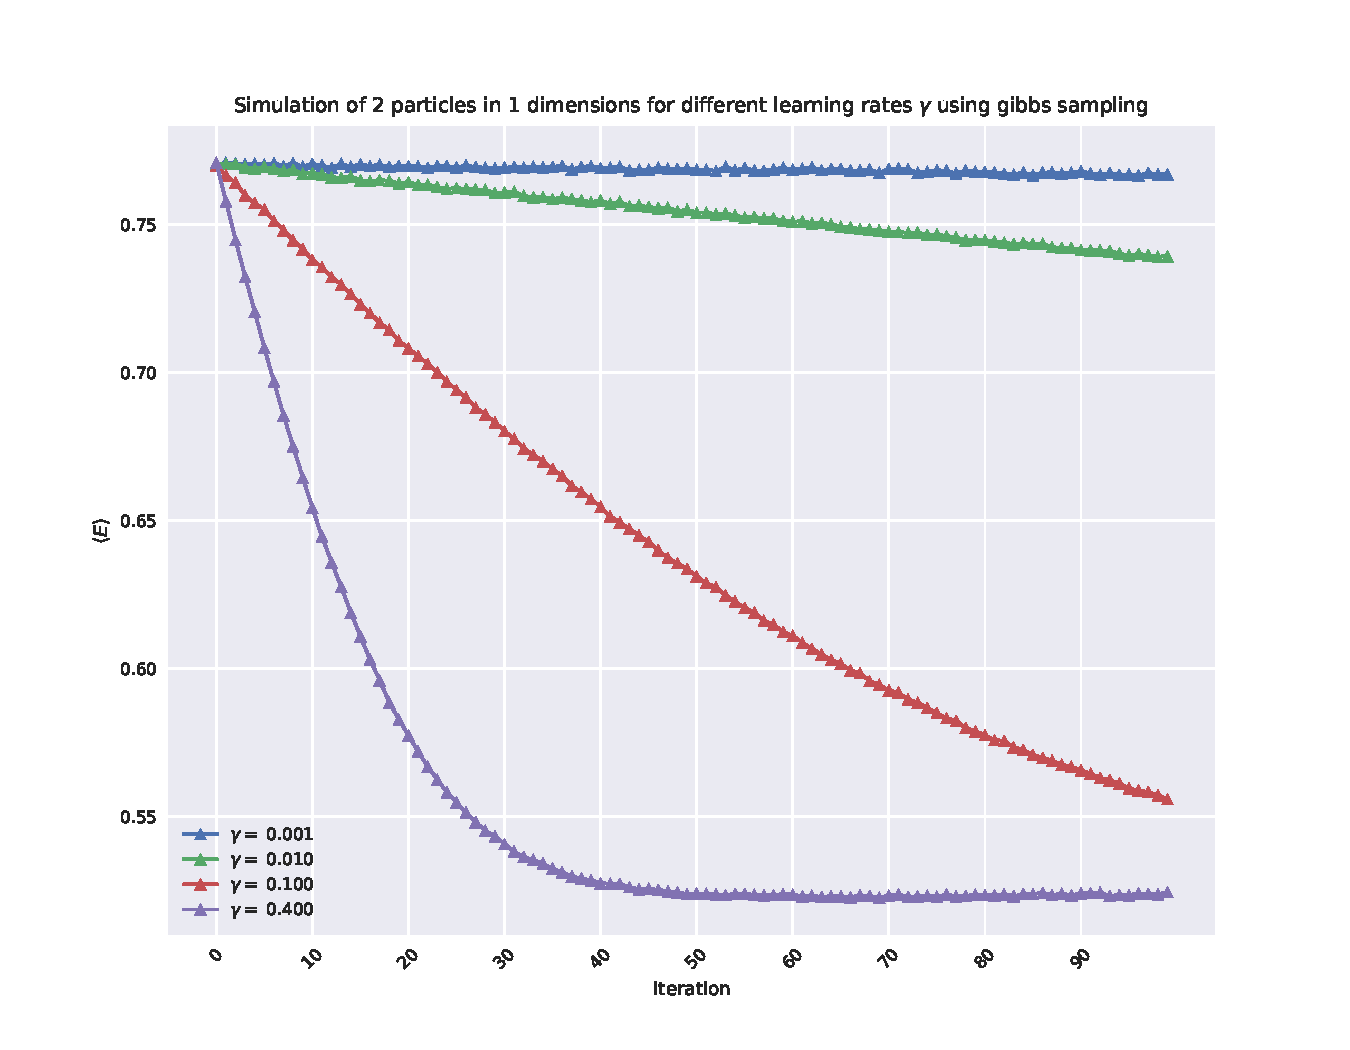
\includegraphics[width = 0.5\paperwidth]{figures/gibbs_2p_1d_N3.pdf} & 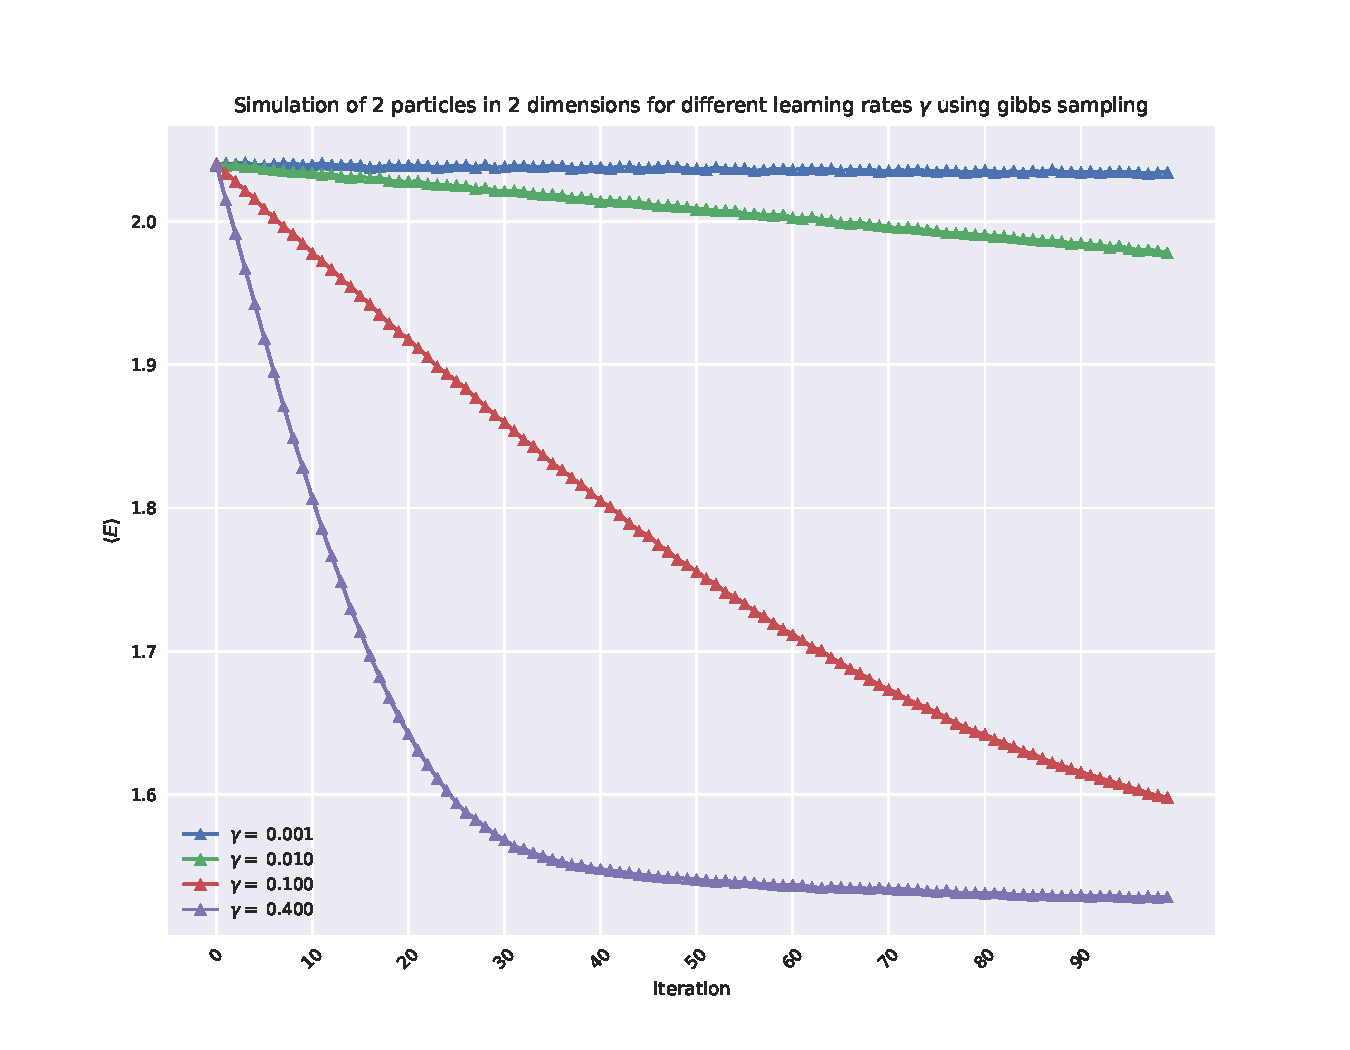
\includegraphics[width = 0.5\paperwidth]{figures/gibbs_2p_2d_N4.pdf} \\
\multicolumn{2}{c}{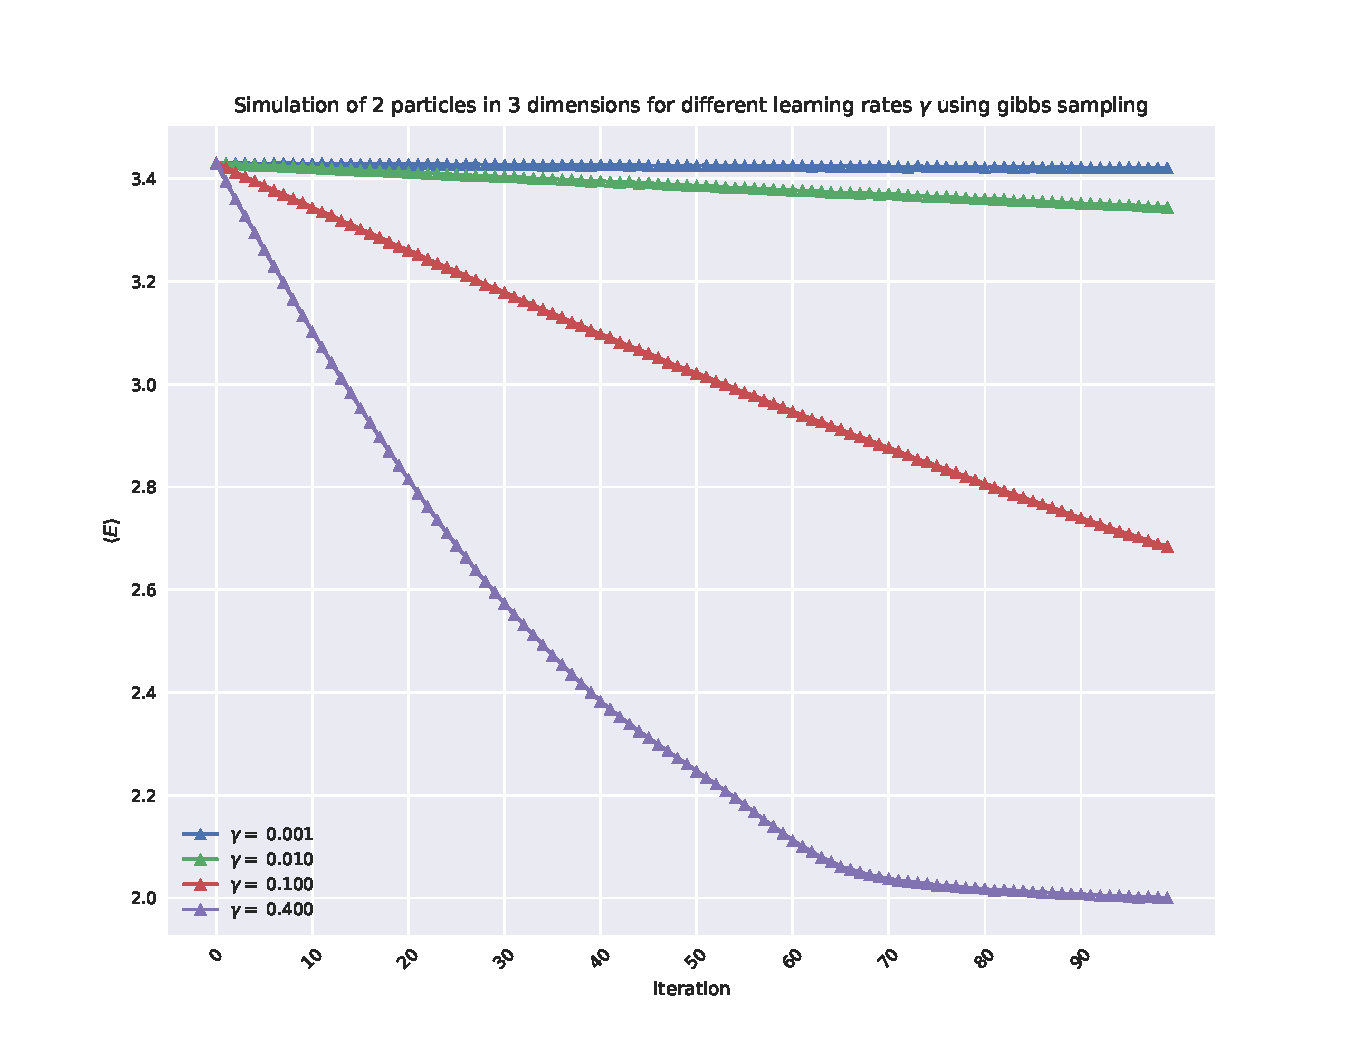
\includegraphics[width=0.5\paperwidth]{figures/gibbs_2p_3d_N8.pdf} }
\end{tabular}
\caption{Plots for simulations with 2 particle and 1-3 dimensions using Gibbs sampling with different training rate values. Number of simulations for optimizing parameters are showed in x-axis.}
\label{fig:1f_2}
\end{figure}

\begin{figure}
\hspace{-2.8cm}
\begin{tabular}{c}
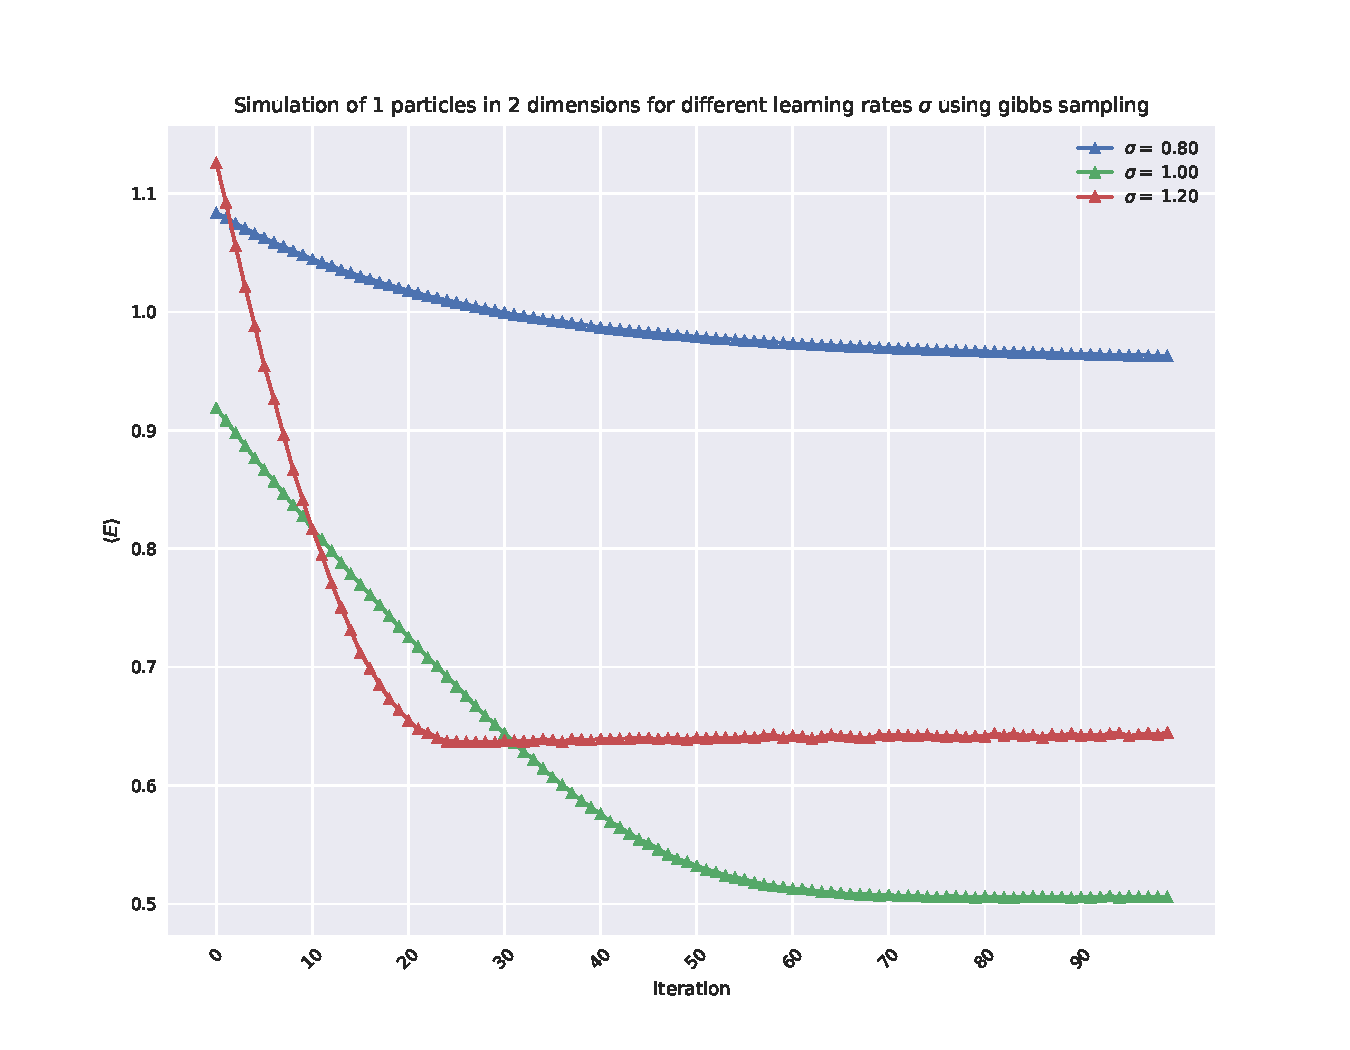
\includegraphics[width = 1.0\paperwidth]{figures/gibbs_08_1_12_gamma04.pdf}\\
\end{tabular}
\caption{Plot of simulation with 1 particle in 2 dimensions using Gibbs sampling with different standard deviation of the nois of the visible nodes, $\sigma$.}
\label{fig:1f_3}
\end{figure}
